\section{Testing af Hjemmesiden}

\subsection{Hvilke Tests}
\begin{frame}{Testing}
	
	\begin{itemize}
	\item	To bruger test sessions
		\begin{itemize}
			\item Finde fejl og problemer ved designet
			\item Midtvejs undersøgelse, så problemerne kan løses i kommende sprints.
			\item Afsluttende tests for at finde stadige problemer, samt at modtage holdninger til fremtidig brug af hjemmesiden.
		\end{itemize}
	\item 	Black-Box Unit Tests
	
	\end{itemize}
	
\end{frame}

\begin{frame}{Brugertests}
	\subsection{Udførelse}
	
	\begin{itemize}
		\item Opgaver 
		\item Tænke højt
		\item Notater
		\item Video		
	\end{itemize}
	
	Udbytte af testene:
	\begin{itemize}
		\item Design fejl
		\item Design problemer
		\item Bedømmelse af hjemmesiden
	\end{itemize}
	
\end{frame}


\begin{frame}{Forside}
	\subsection{Forbedringer}
	
	\begin{minipage}[0.3\textheight]{\textwidth}
	\begin{columns}[T]
	\begin{column}{0.5\textwidth}
	\begin{itemize}
	\item Farve tema skiftet
	\item Mere indbydende
	\item Tilføjet en reel forside.
	
	\end{itemize}
	\end{column}
	\begin{column}{0.5\textwidth}
	 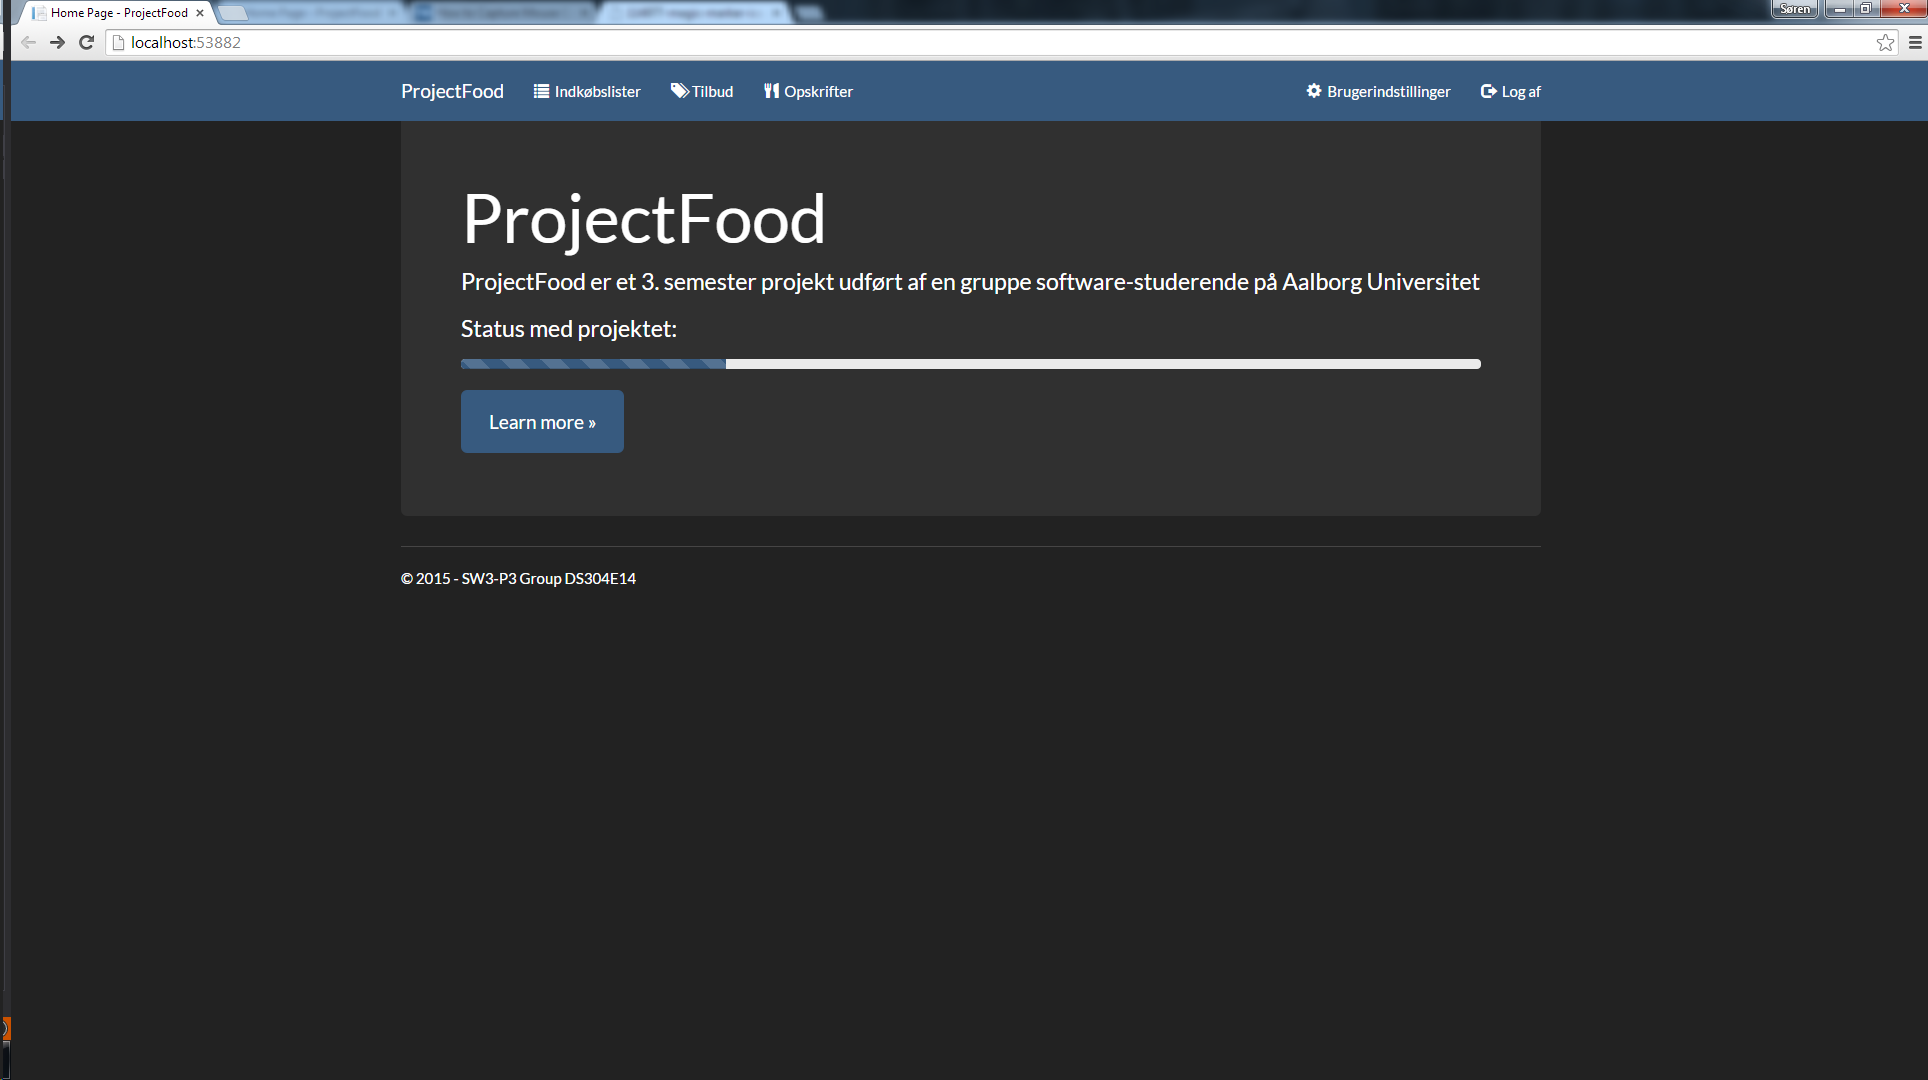
\includegraphics[width=0.9\textwidth,height=0.8\textheight,keepaspectratio]{images/Screenshots/FrontPageOld.png}
	 
	 \vspace{2 mm}
	  
	  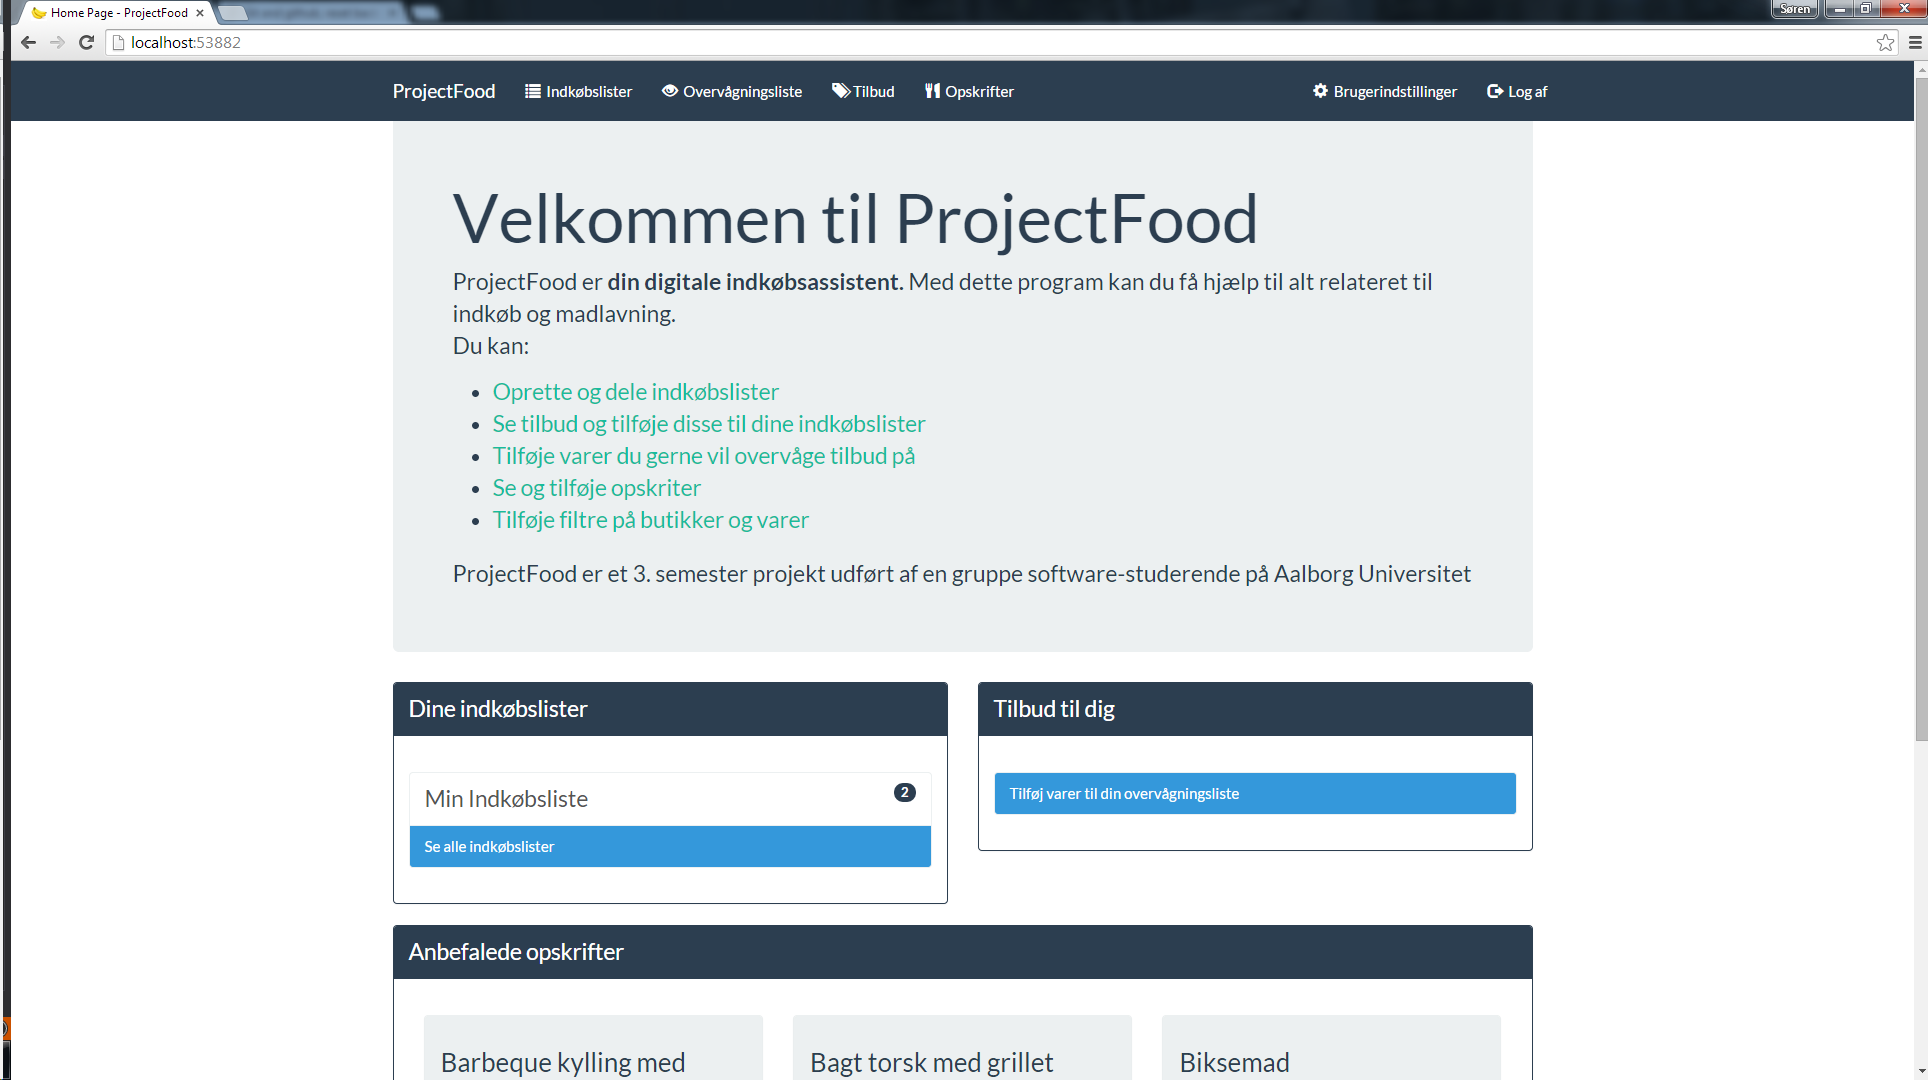
\includegraphics[width=0.9\textwidth,height=0.8\textheight,keepaspectratio]{images/Screenshots/FrontPage.png}
	\end{column}
	\end{columns}
	

  \end{minipage}
	
\end{frame}

\begin{frame}{Indstillinger}
	
	\begin{minipage}[0.3\textheight]{\textwidth}
	\begin{columns}[T]
	\begin{column}{0.5\textwidth}
	 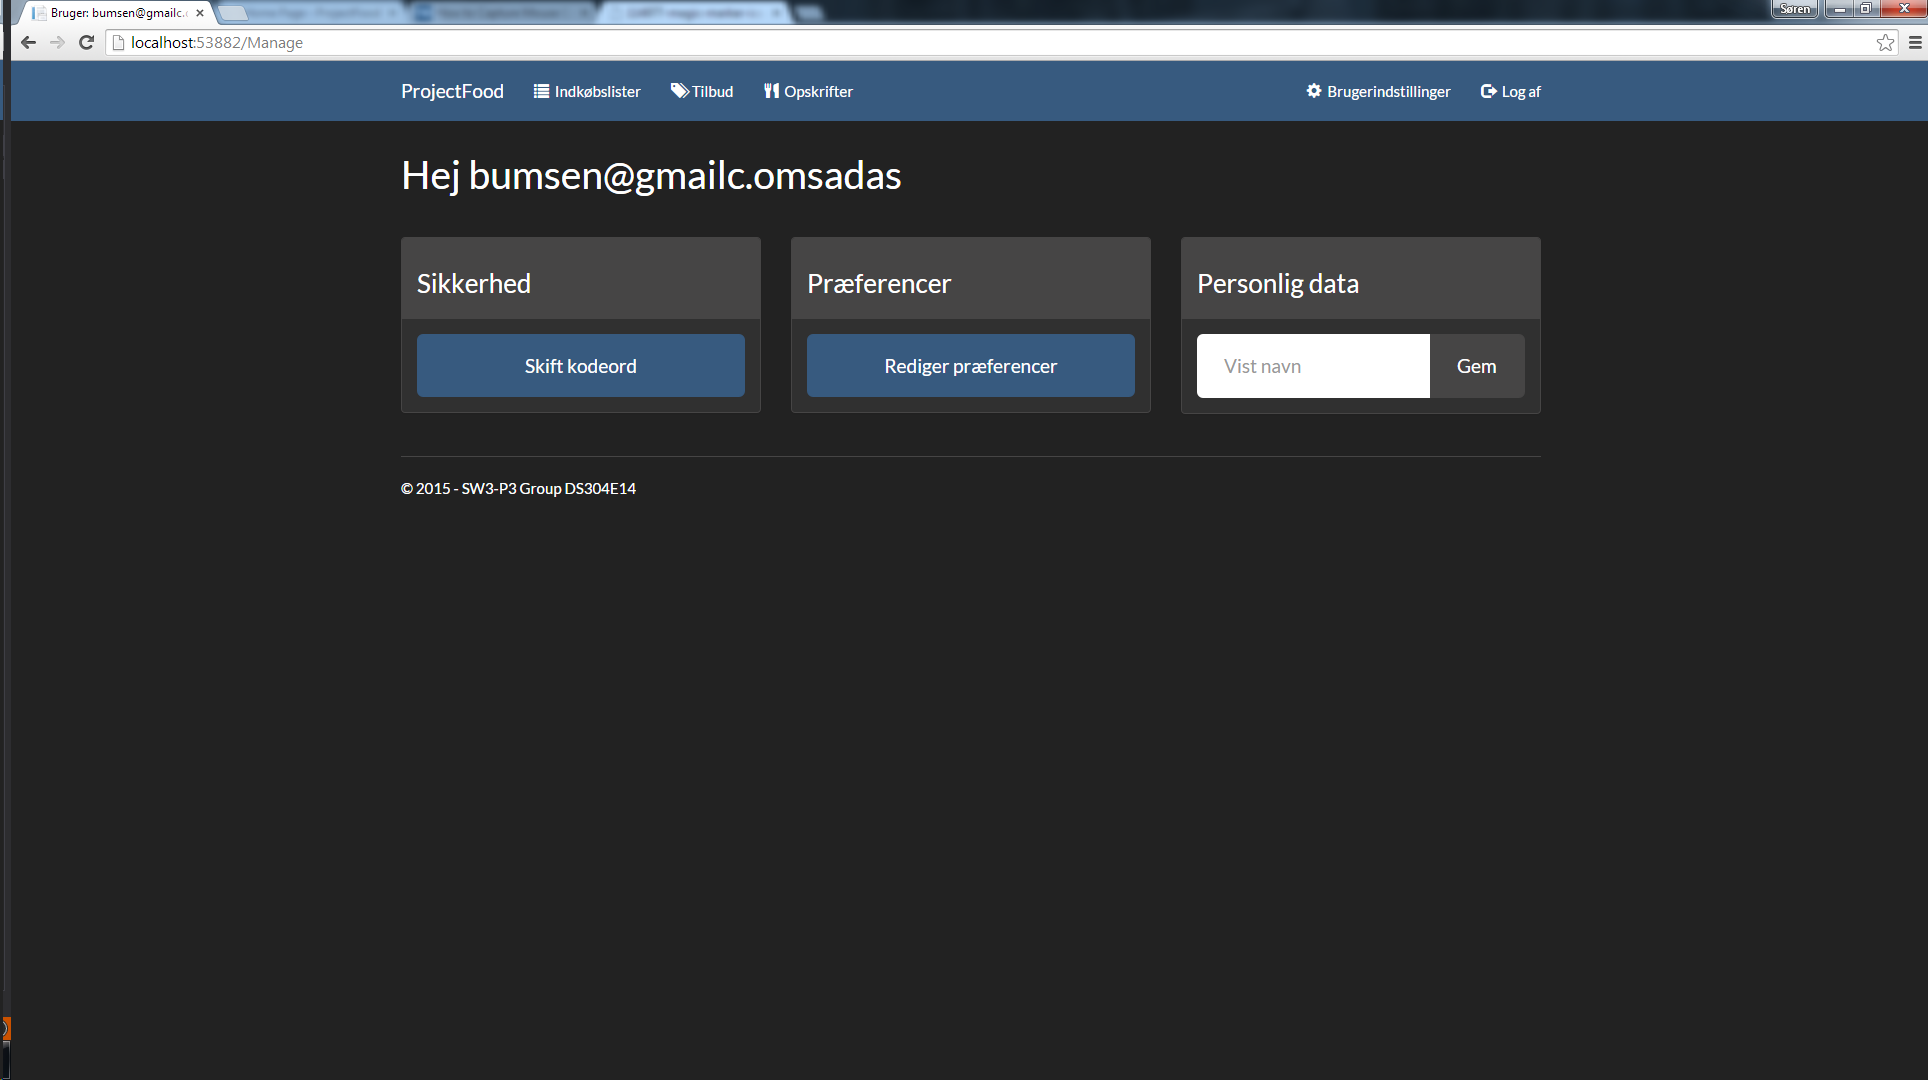
\includegraphics[width=0.9\textwidth,height=0.8\textheight,keepaspectratio]{images/Screenshots/SettingsOld.png} \vspace{2 mm} $\rightarrow$ 
	 
	 \begin{itemize}
	 	\item Reduceret antal klik
	 	\item Fjernet ordet Præferencer
	 	\item Forsøgt at give feedback
	 \end{itemize}
	 
	\end{column}
	\begin{column}{0.5\textwidth}
	 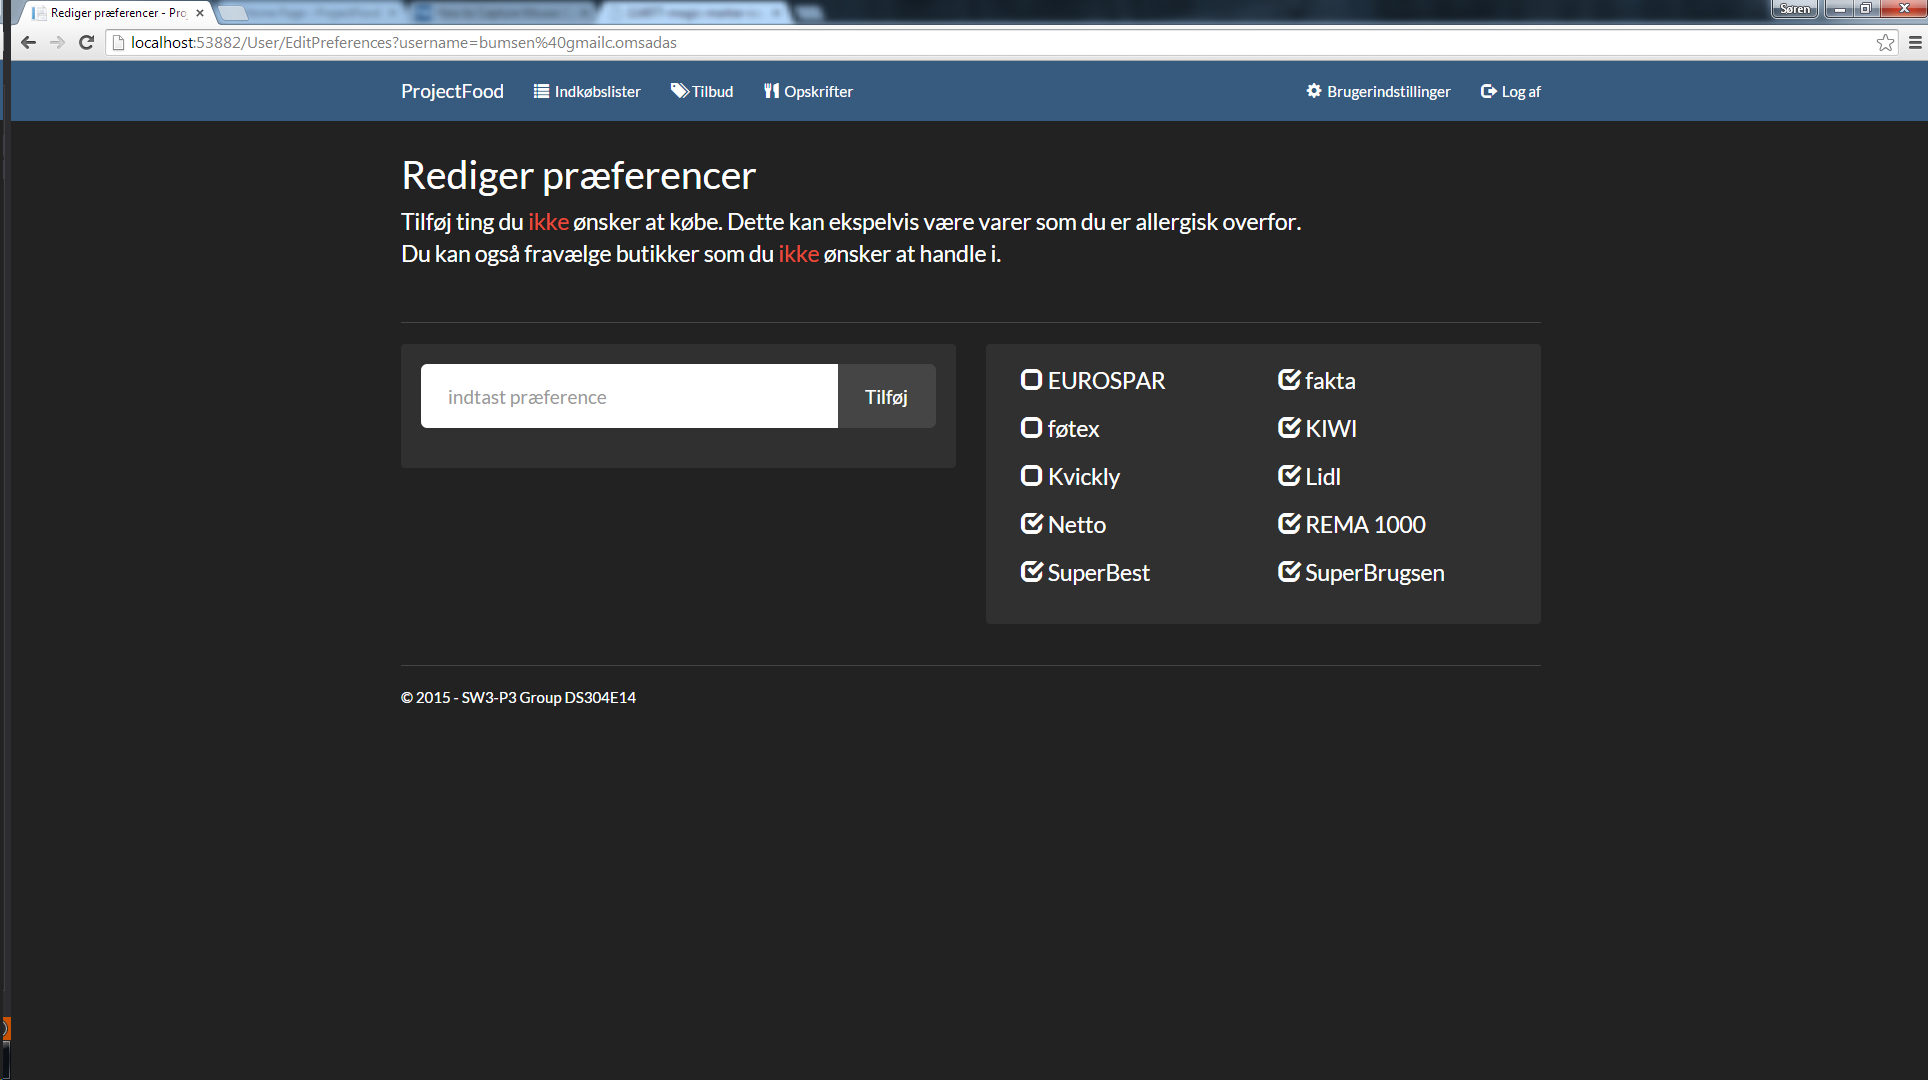
\includegraphics[width=0.9\textwidth,height=0.8\textheight,keepaspectratio]{images/Screenshots/SettingsOld2.png}
	 
	 \vspace{2 mm}
	  
	  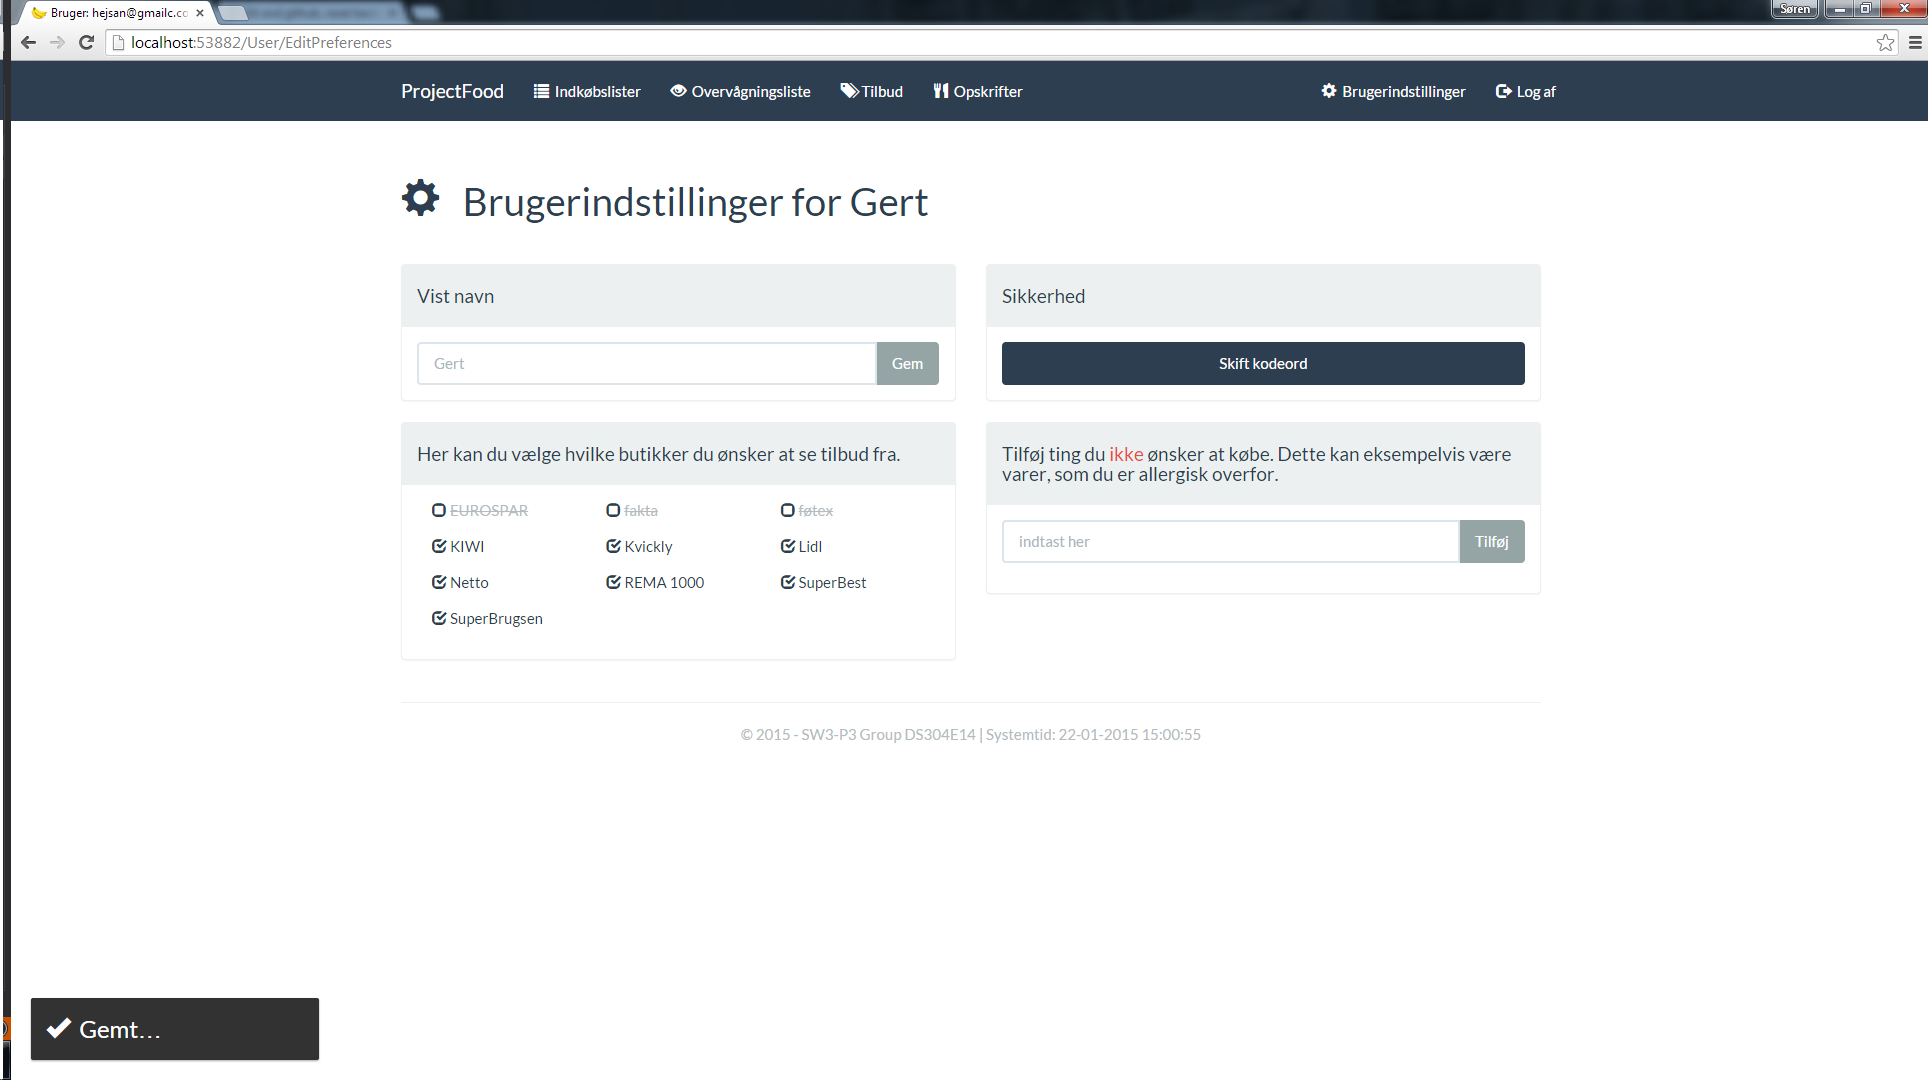
\includegraphics[width=0.9\textwidth,height=0.8\textheight,keepaspectratio]{images/Screenshots/Settings.png}
	\end{column}
	\end{columns}
	

  \end{minipage}
	
\end{frame}

\begin{frame}{Indkøbsliste}
	
	\begin{minipage}[0.3\textheight]{\textwidth}
	\begin{columns}[T]
	\begin{column}{0.5\textwidth}
	 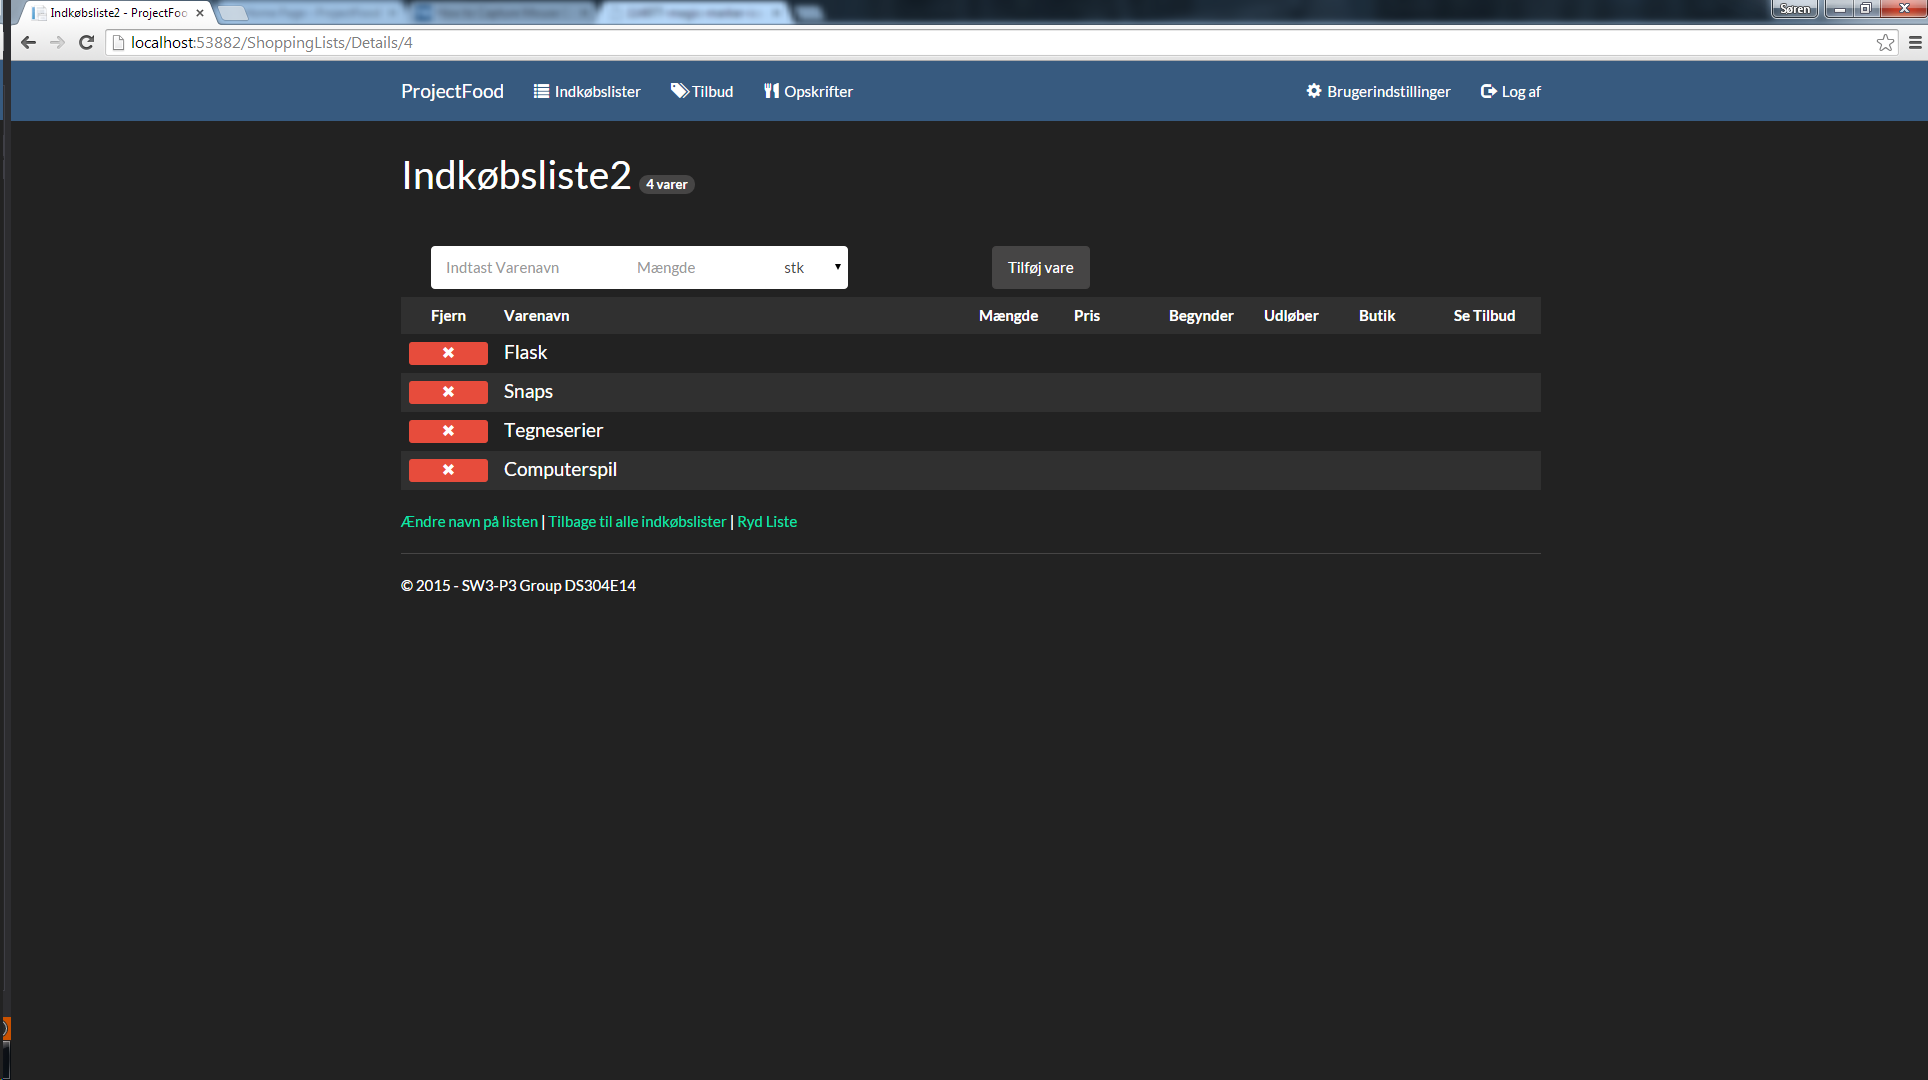
\includegraphics[width=0.9\textwidth,height=0.8\textheight,keepaspectratio]{images/Screenshots/ShoppingListOld.png}
	 
	 \begin{itemize}
	 	\item Viser altid ikon nu
	 	\item Adskillelse af input bokse
	 	\item Konsistente farver for vælg tilbud
	 \end{itemize}
	 
	\end{column}
	\begin{column}{0.5\textwidth}
	 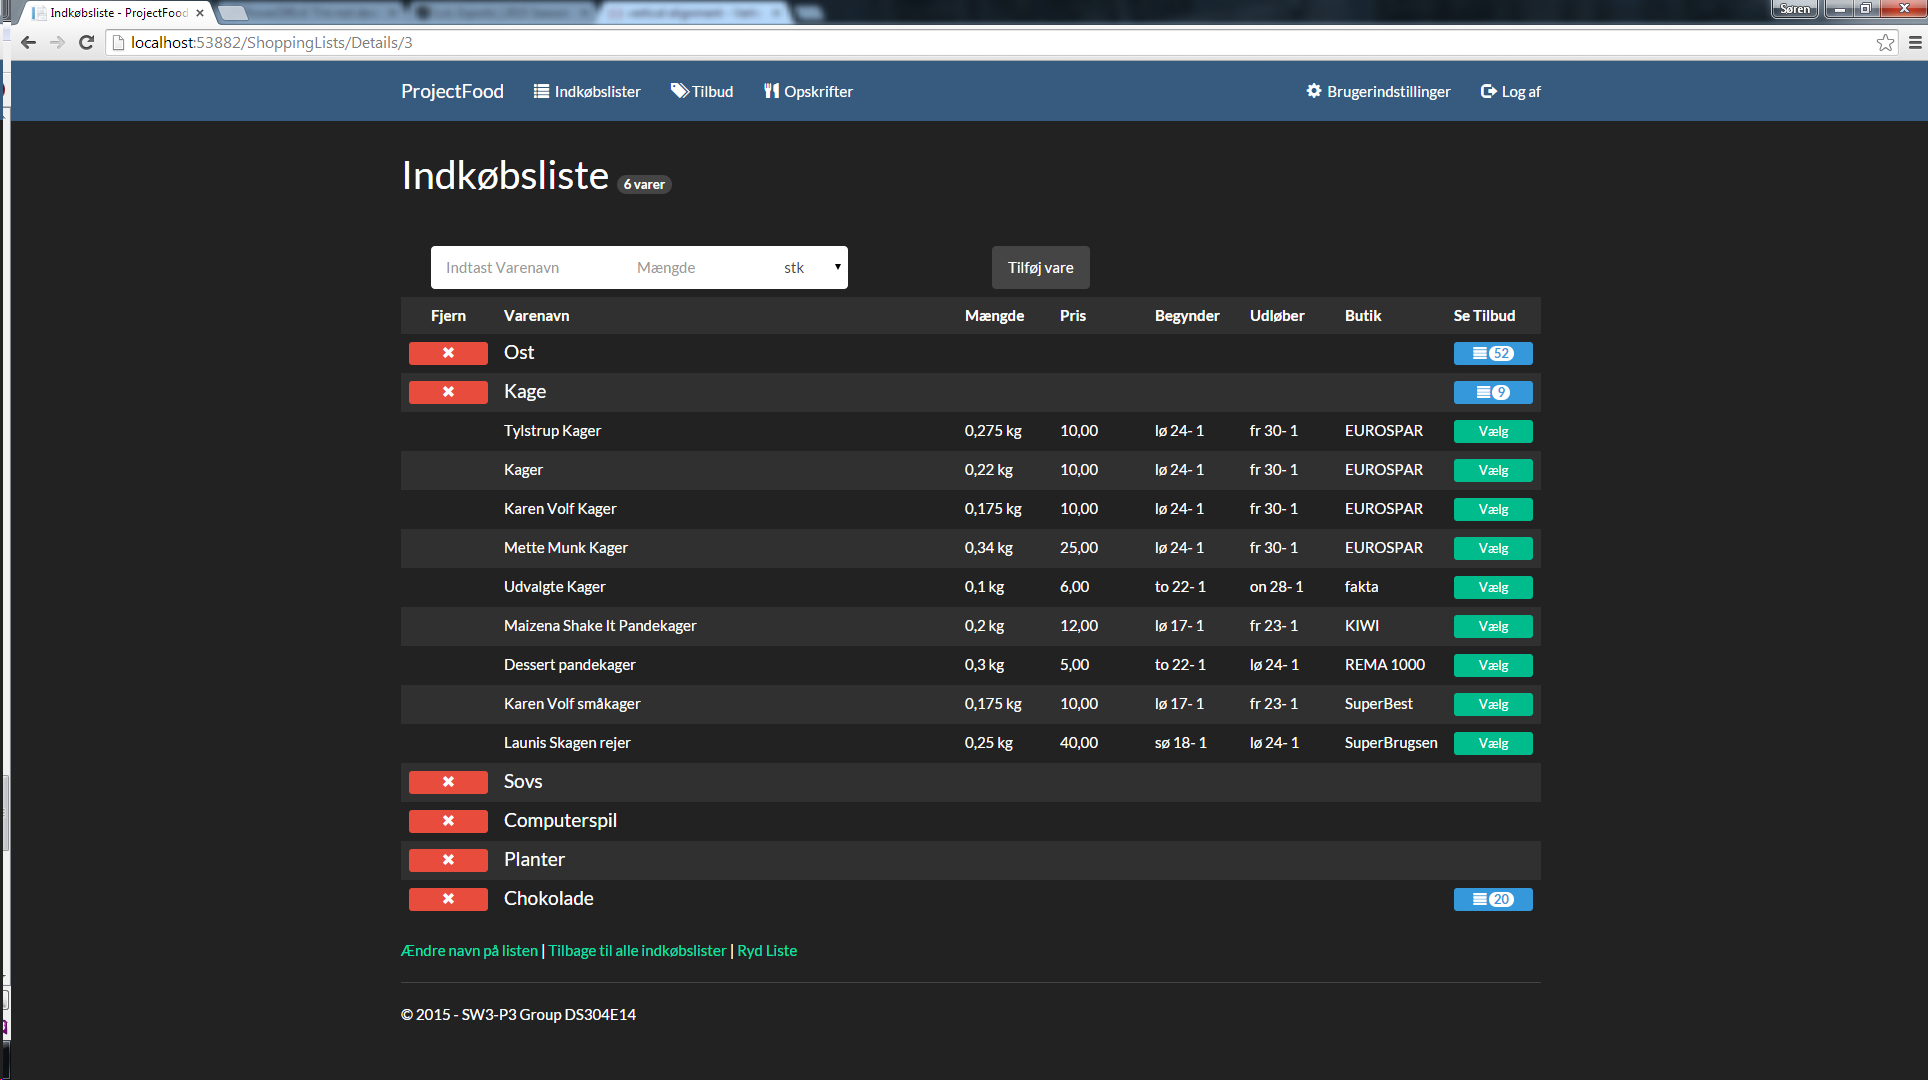
\includegraphics[width=0.9\textwidth,height=0.8\textheight,keepaspectratio]{images/Screenshots/ShoppingListOffersOld.png}
	 
	 \vspace{2 mm}
	  
	  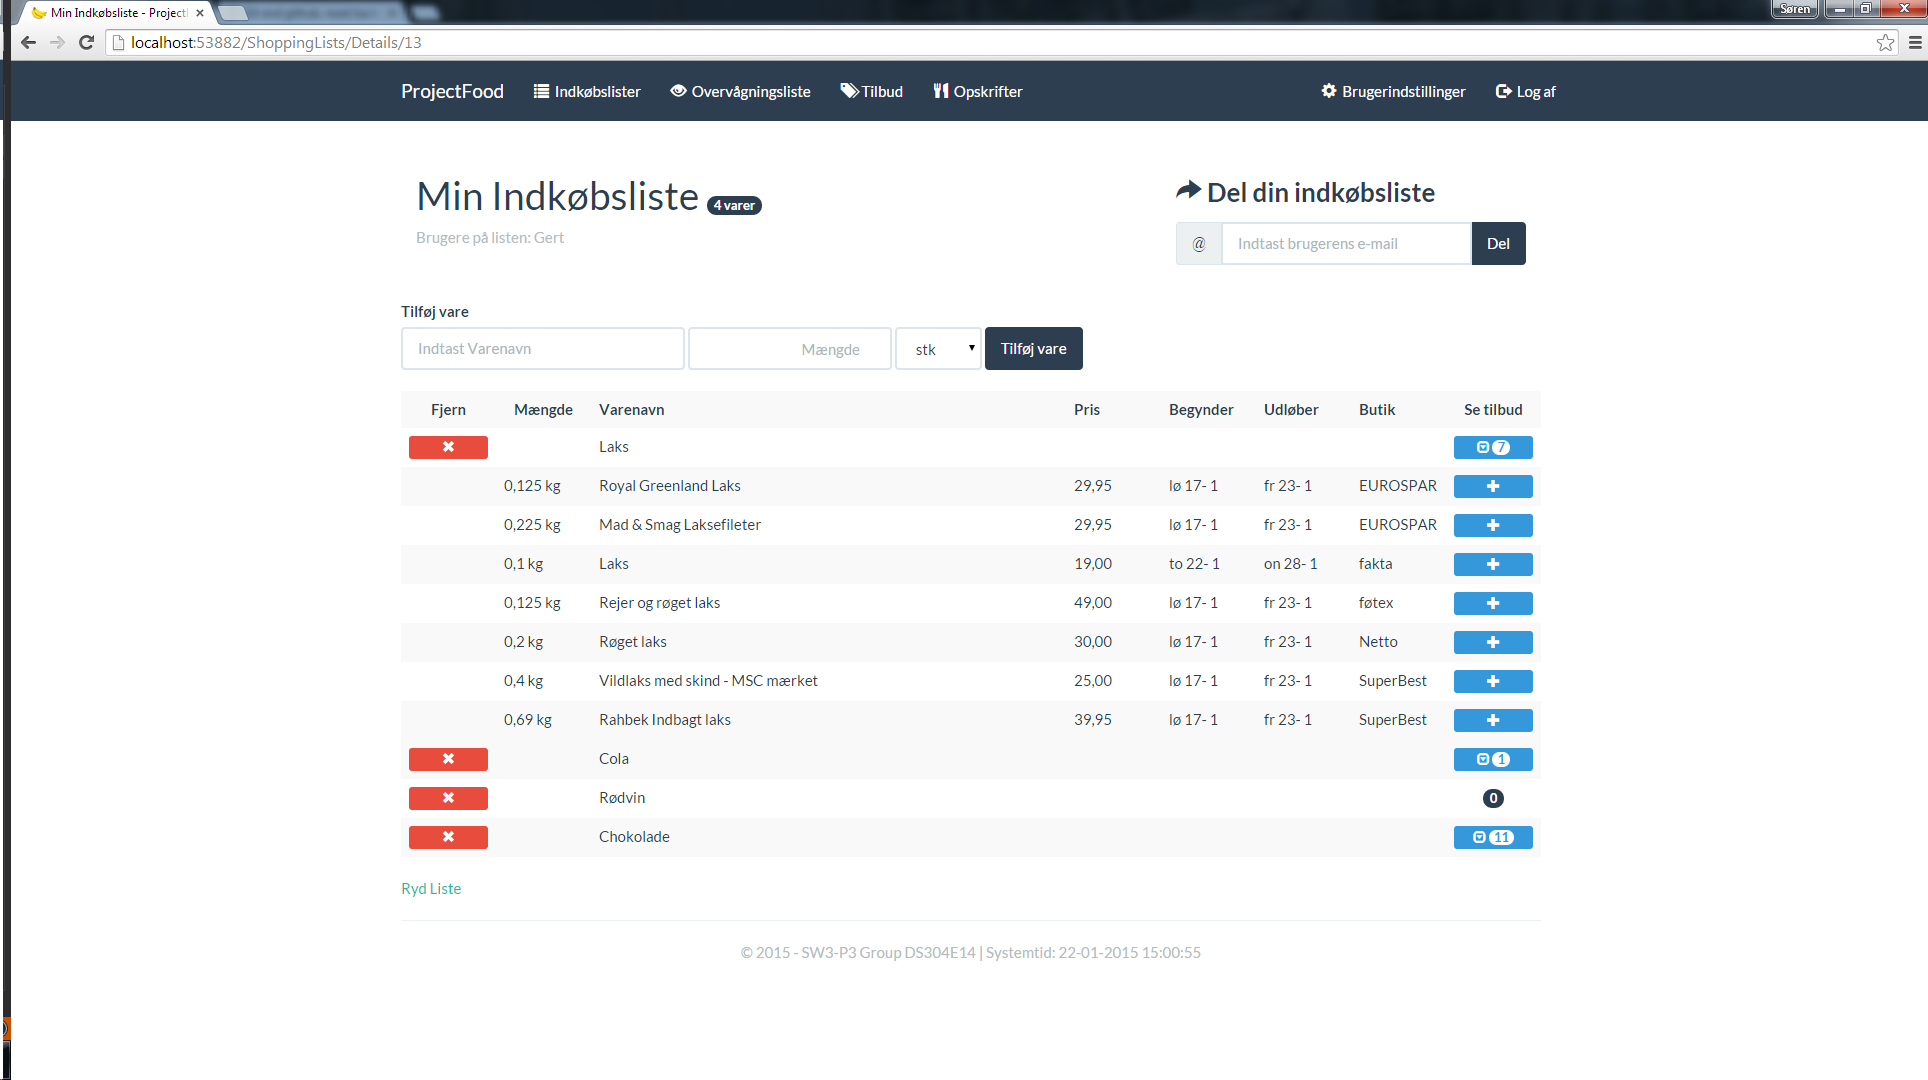
\includegraphics[width=0.9\textwidth,height=0.8\textheight,keepaspectratio]{images/Screenshots/ShoppingList.png}
	\end{column}
	\end{columns}
	

  \end{minipage}
	
\end{frame}

\begin{frame}{Tilbud}
	
	\begin{minipage}[0.3\textheight]{\textwidth}
	\begin{columns}[T]
	\begin{column}{0.5\textwidth}
	\begin{itemize}
	\item Flyttet vælg indkøbsliste
	\item Paginering for større overblik

	
	\end{itemize}
	\end{column}
	\begin{column}{0.5\textwidth}
	 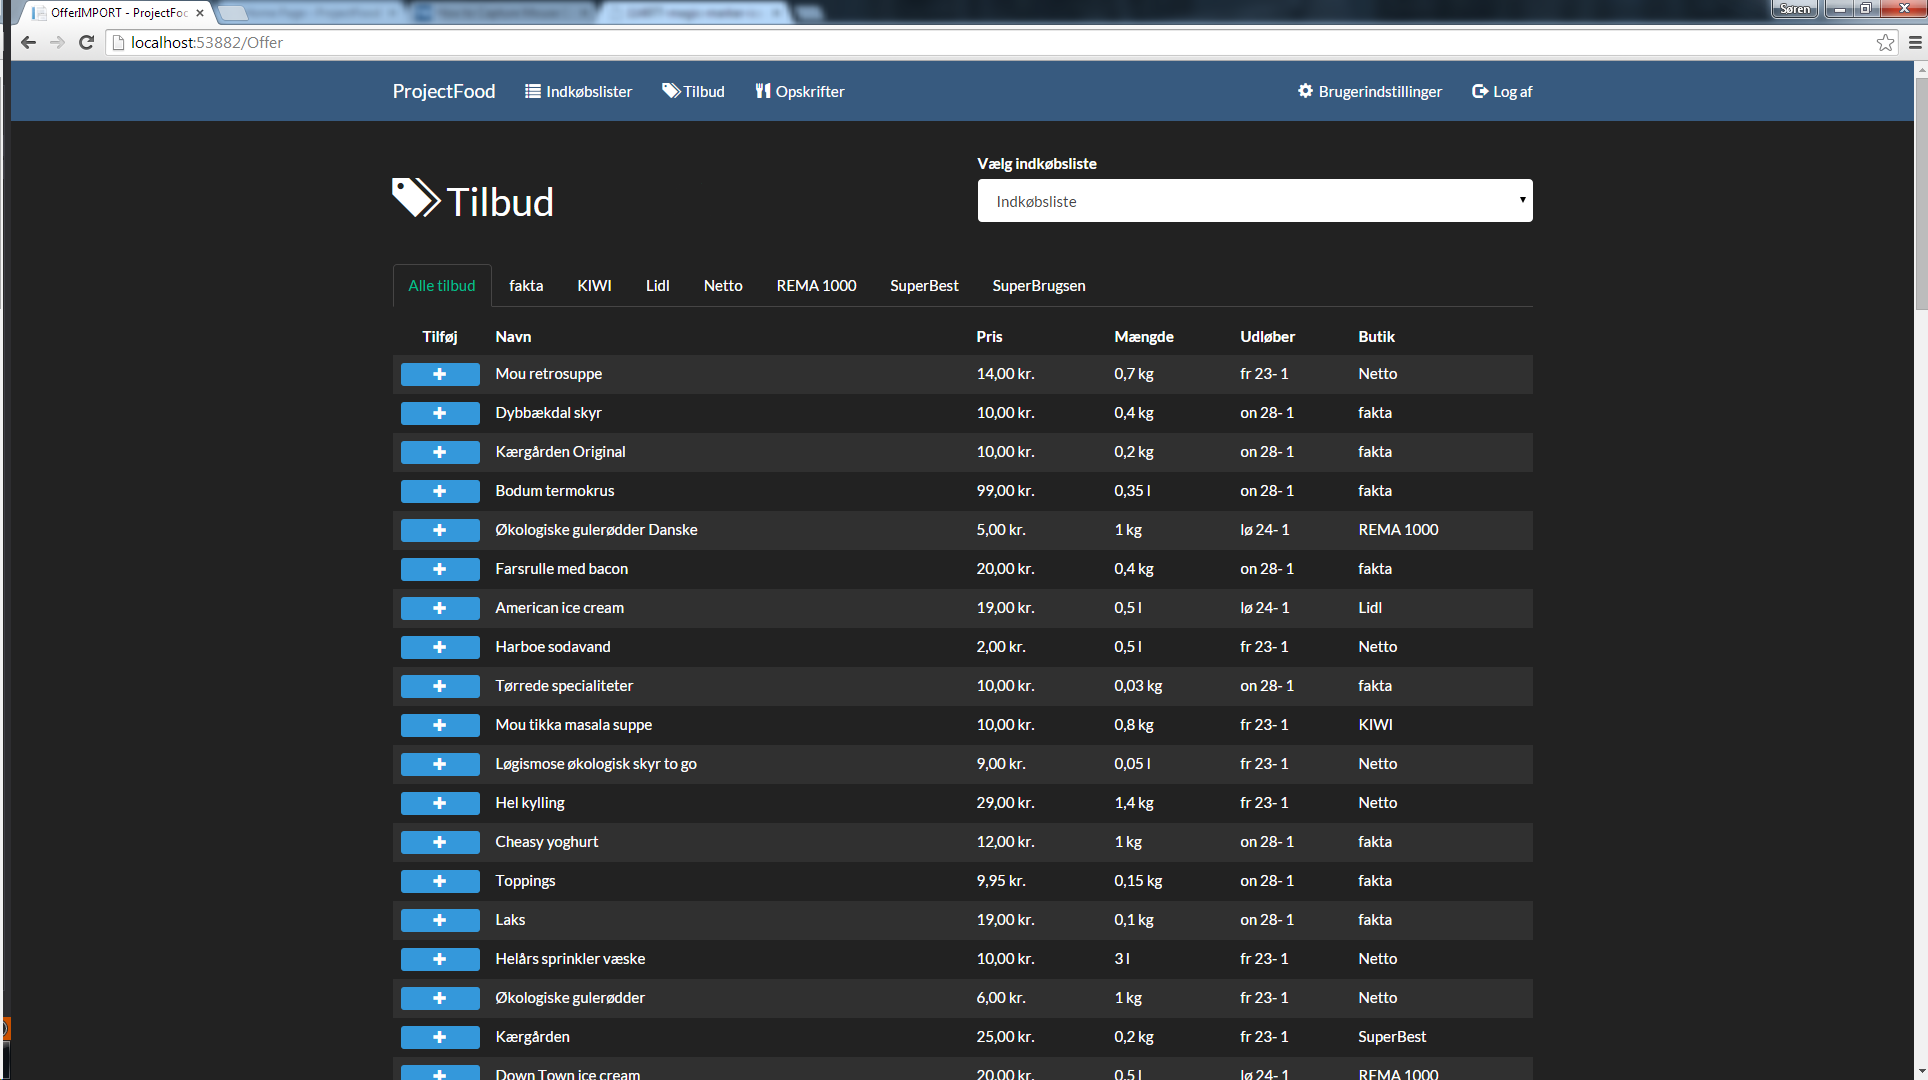
\includegraphics[width=0.9\textwidth,height=0.8\textheight,keepaspectratio]{images/Screenshots/OffersOld.png}
	 
	 \vspace{2 mm}
	  
	  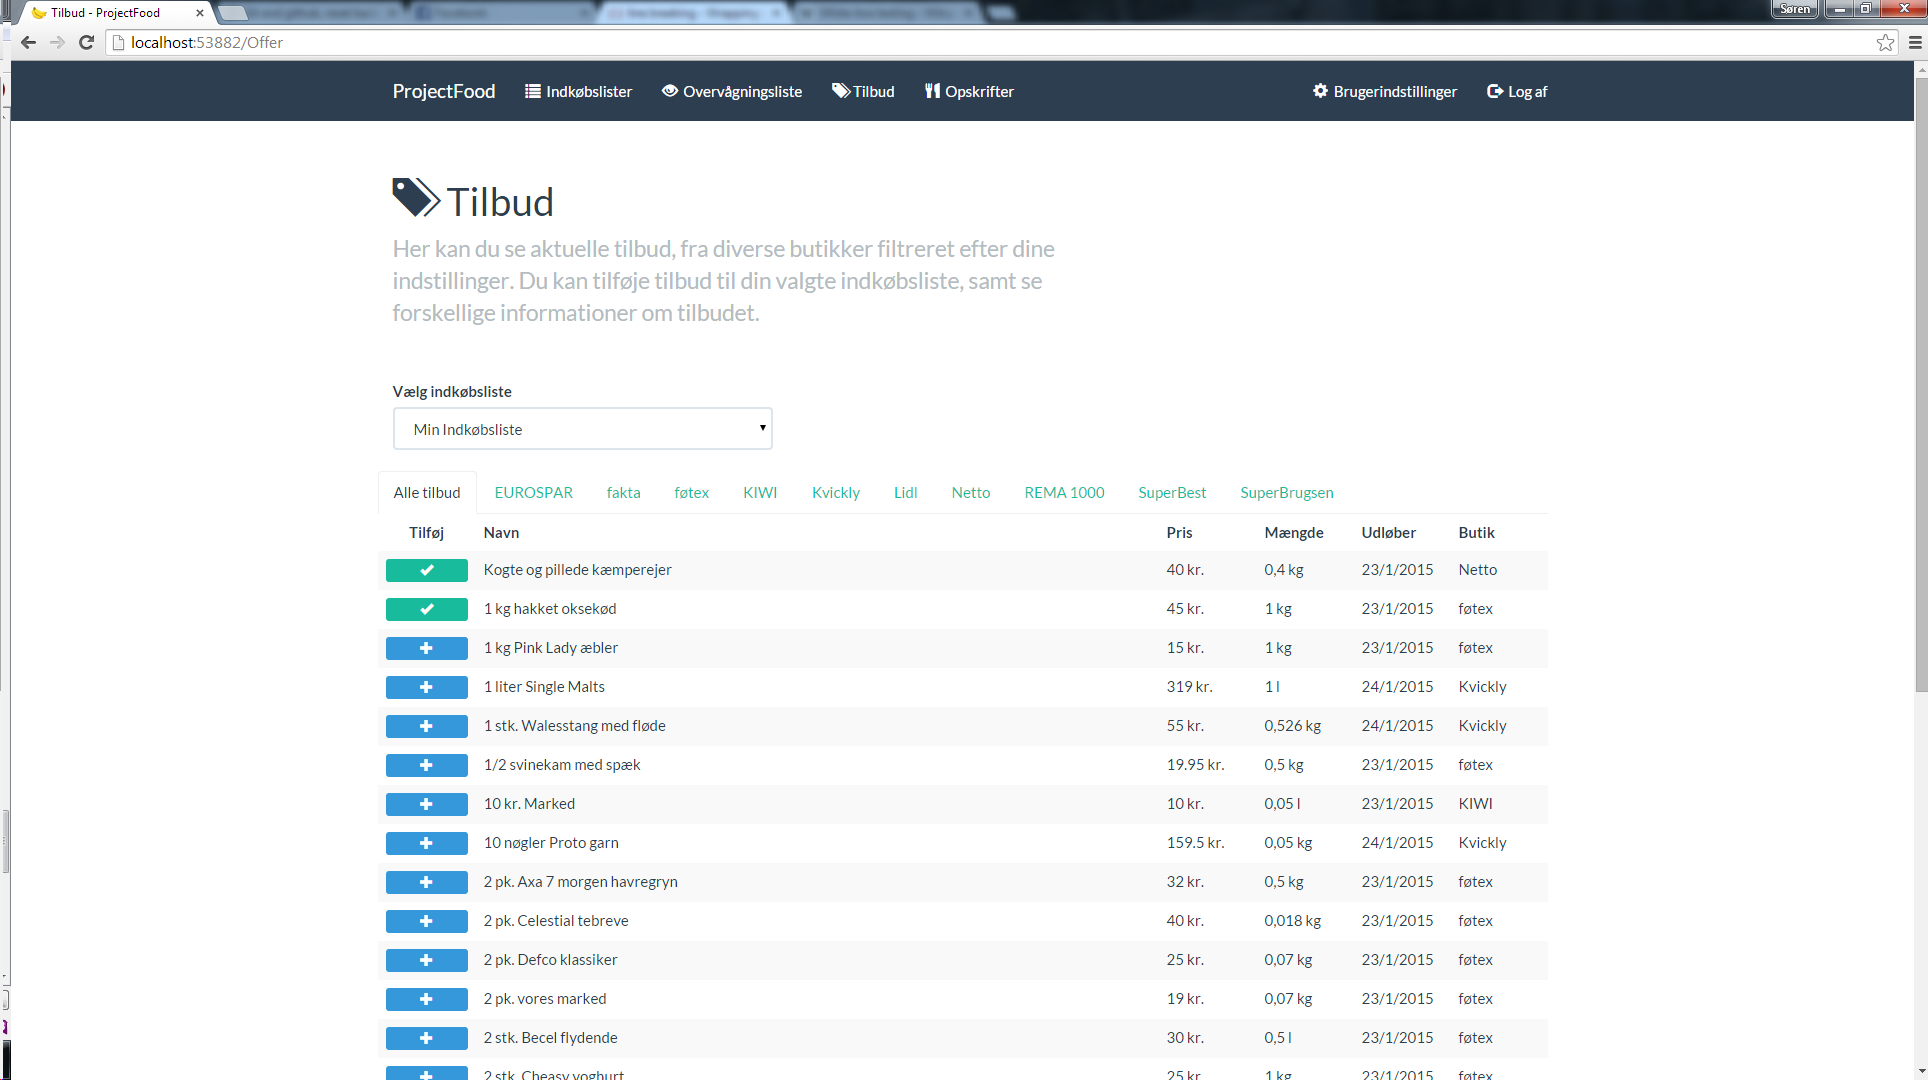
\includegraphics[width=0.9\textwidth,height=0.8\textheight,keepaspectratio]{images/Screenshots/Offers.png}
	\end{column}
	\end{columns}
	

  \end{minipage}
  
  	
\end{frame}
\begin{frame}{Opskrifter}
	
	\begin{minipage}[0.3\textheight]{\textwidth}
	\begin{columns}[T]
	\begin{column}{0.5\textwidth}
	\begin{itemize}
	\item Mouseover
	\item Ingen kunne navigere ind på opskriften uden først at blive i tvivl om hvordan.

	
	\end{itemize}
	\end{column}
	\begin{column}{0.5\textwidth}
	 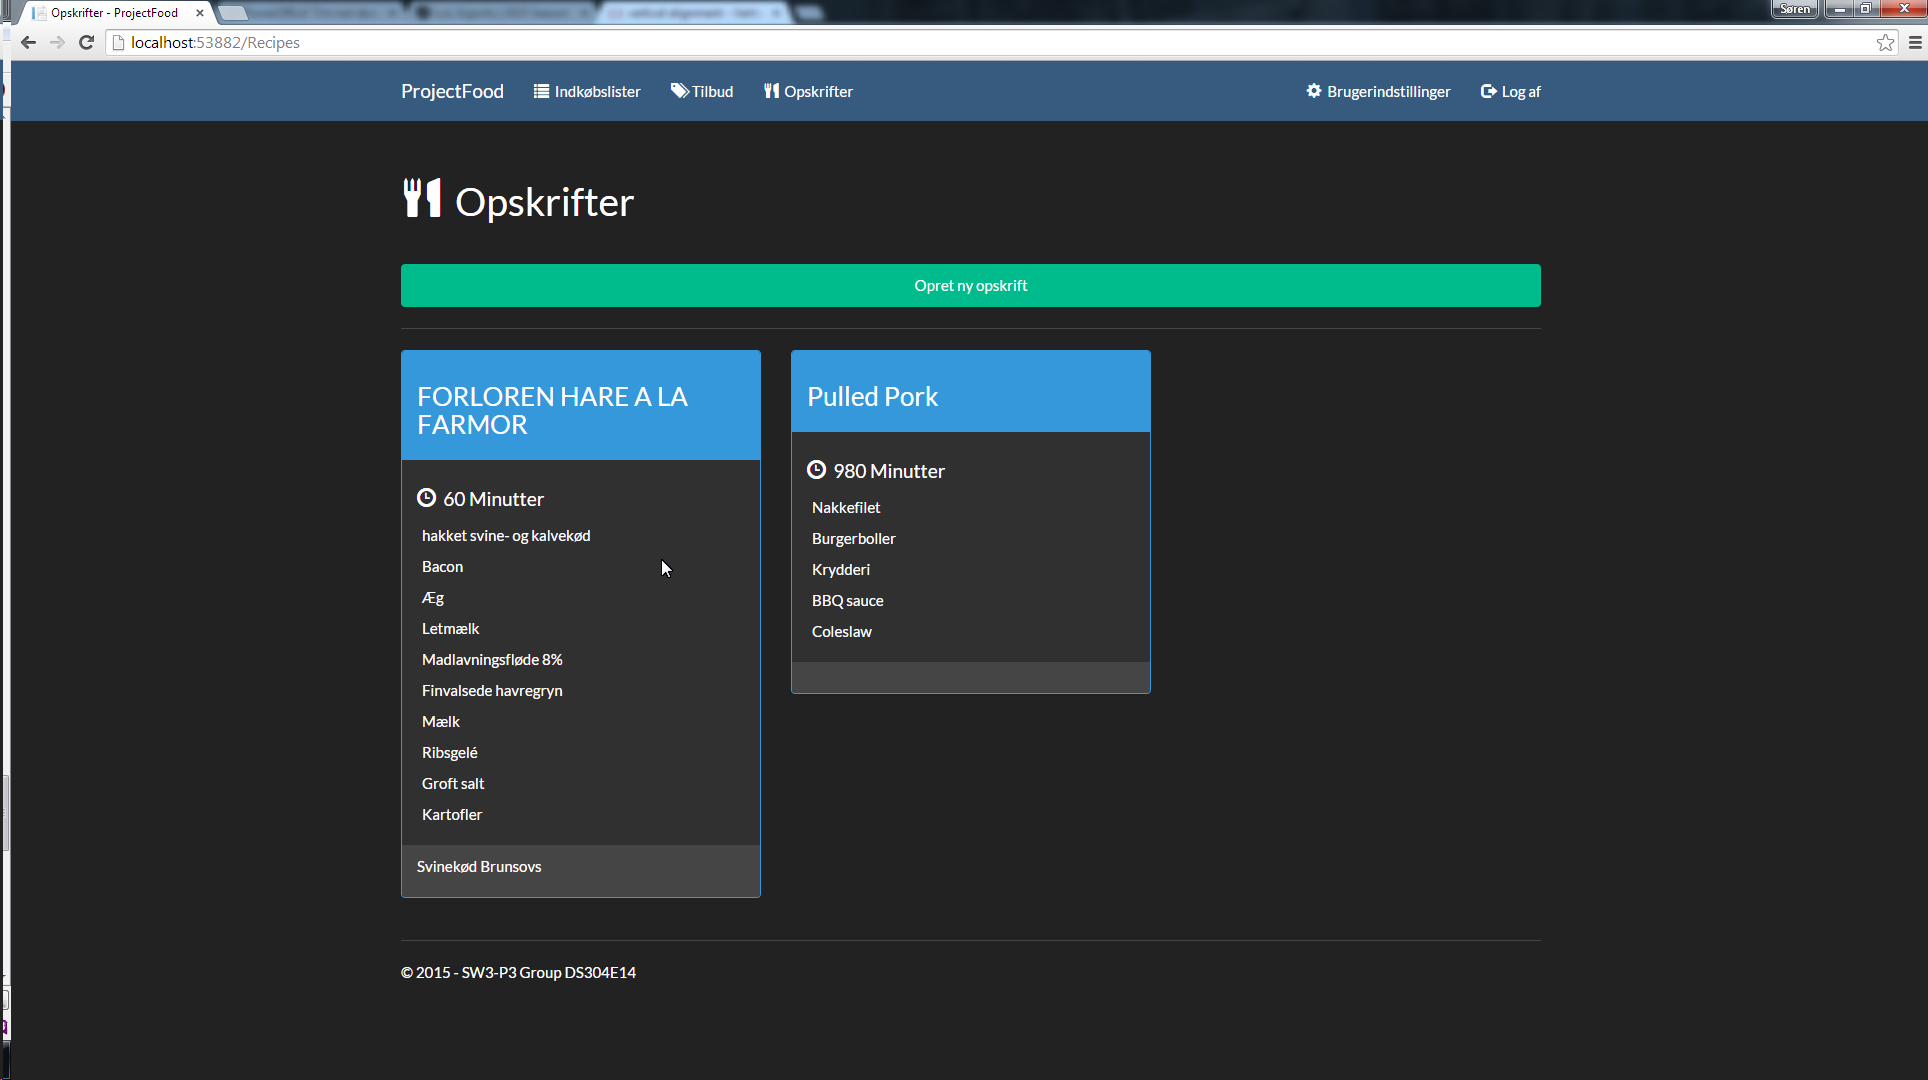
\includegraphics[width=0.9\textwidth,height=0.8\textheight,keepaspectratio]{images/Screenshots/RecipeOld.png}
	 
	 \vspace{2 mm}
	  
	  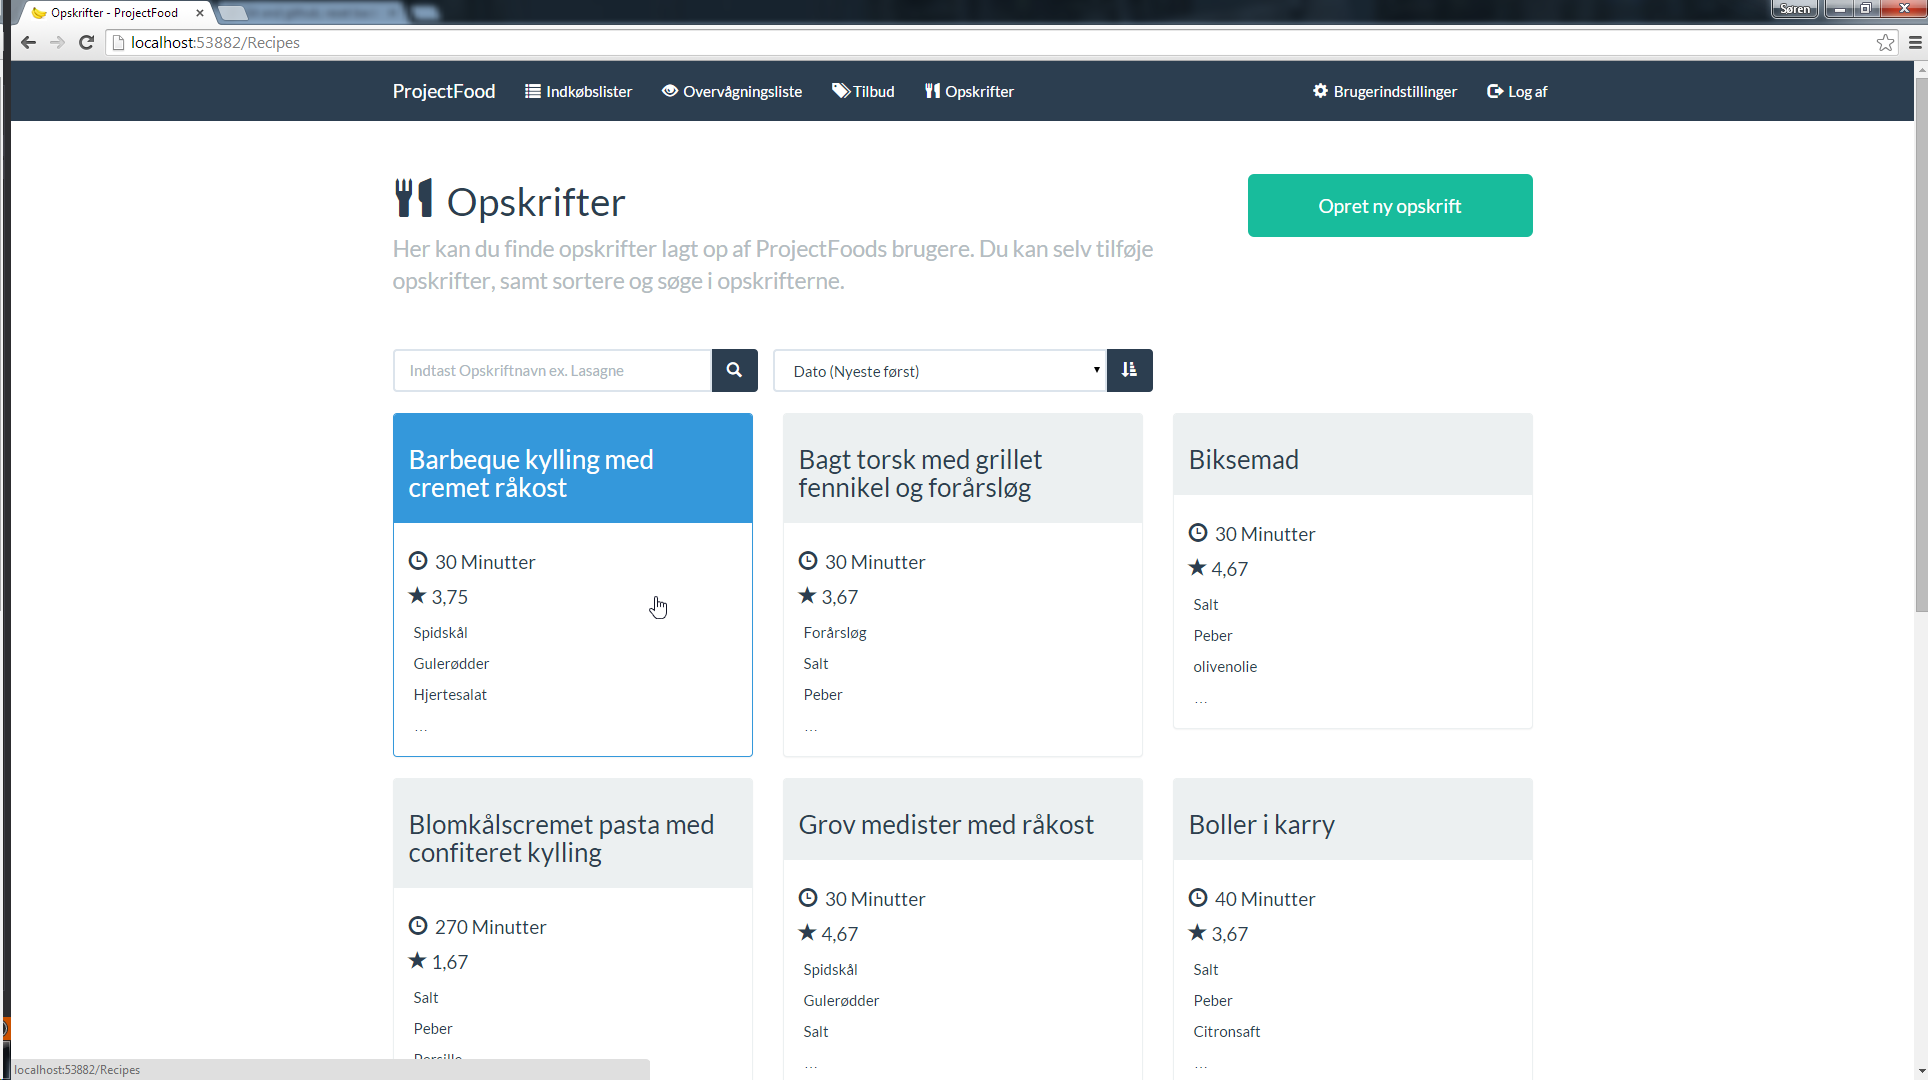
\includegraphics[width=0.9\textwidth,height=0.8\textheight,keepaspectratio]{images/Screenshots/Recipe.png}
	\end{column}
	\end{columns}
	

  \end{minipage}
  
  	
\end{frame}

\begin{frame}{Opskrifter}
	
	\begin{minipage}[0.3\textheight]{\textwidth}
	\begin{columns}[T]
	\begin{column}{0.5\textwidth}
	\begin{itemize}
	\item Gruppering af elementer der er fælles
	\item Tilføjet funktion til at tilføje alle ingredienser.

	
	\end{itemize}
	\end{column}
	\begin{column}{0.5\textwidth}
	 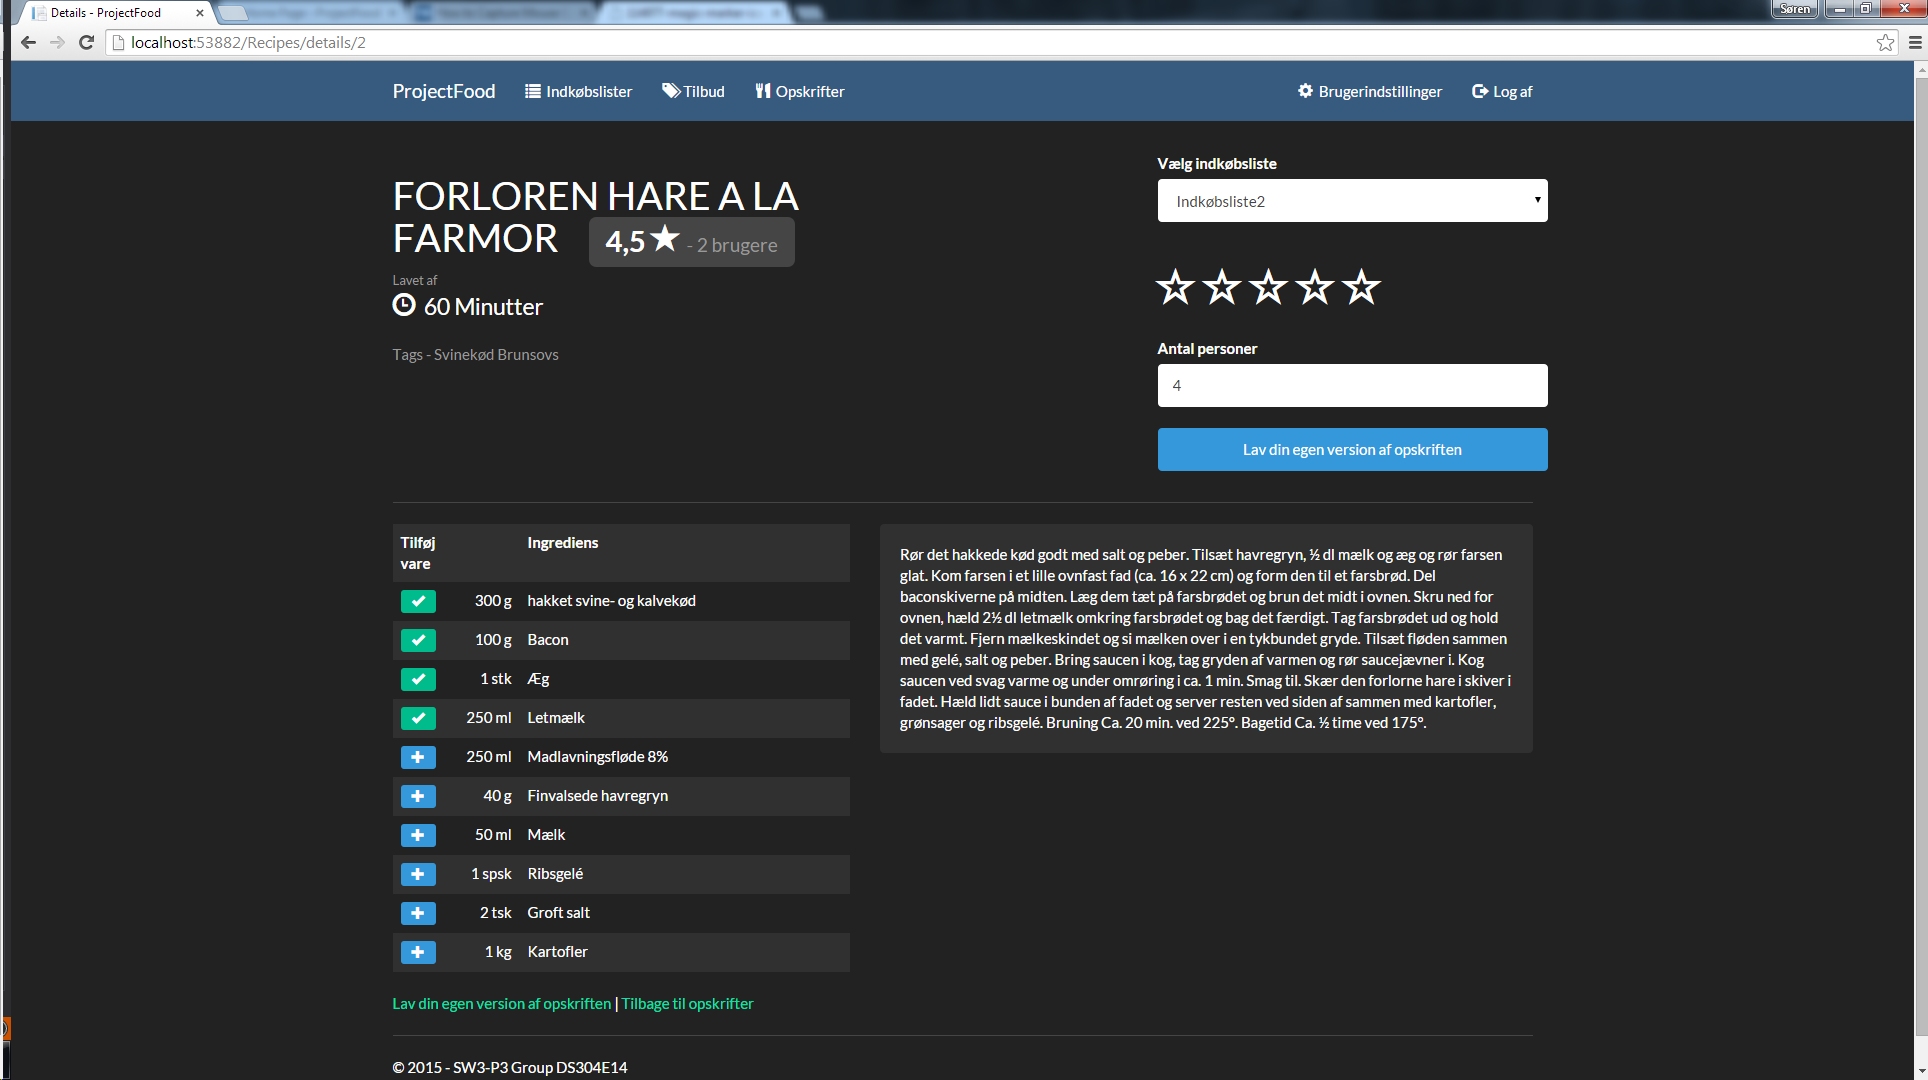
\includegraphics[width=0.9\textwidth,height=0.8\textheight,keepaspectratio]{images/Screenshots/PickedRecipeOld.png}
	 
	 \vspace{2 mm}
	  
	  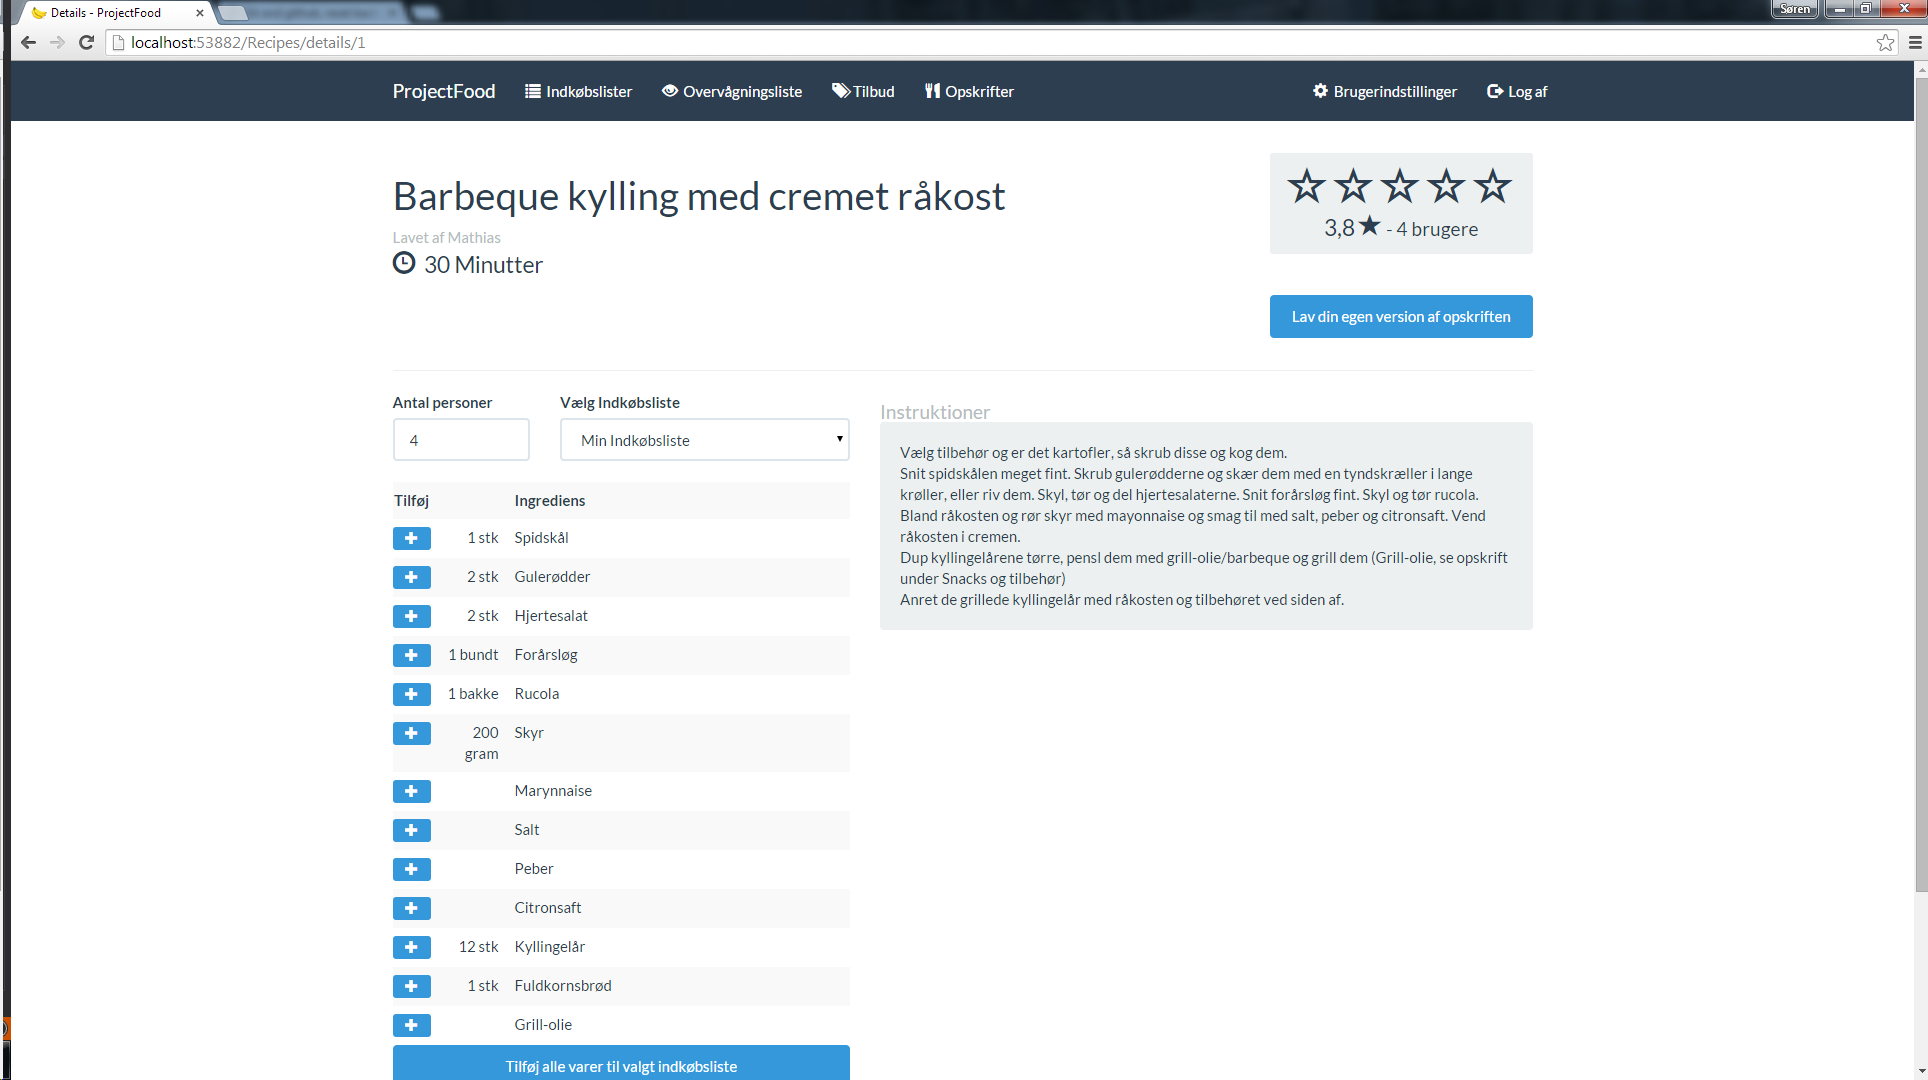
\includegraphics[width=0.9\textwidth,height=0.8\textheight,keepaspectratio]{images/Screenshots/PickedRecipe.png}
	\end{column}
	\end{columns}
	

  \end{minipage}
  
  	
\end{frame}

\begin{frame}{Konklusion på Brugertests}	
	
\begin{itemize}
	\item Vi var ikke gode til at bruge vores design principper.
		\begin{itemize}
			\item Proximity
			\item Feedback
			\item Navigation
			\item Consistency
		\end{itemize}
	\item Mange af problemerne blev udrettet i den endelige udgave
	\item Der var store problemer med Feedback, og Consistency
\end{itemize}
  
\end{frame}


\begin{frame}{Unit Tests}
\subsection{Unit Tests}

Hvorfor unit tests?

Input $\rightarrow$ SomeFunction $\rightarrow$  Output

Coverage

\end{frame}
